%!TEX root = ../MC_SS17.tex
\section{Systemmodellierung durch Automaten}
\label{sec:para2}

Der erste Schritt für das Model-Checking ist die Modellierung des Systems. Dies ist in der Praxis oft schwierig, da das Modell detailliert genug sein muss um interessante Eigenschaften zu erfassen, gleichzeitig aber auch abstrakt genug sein muss, um automatische Verifikation zu ermöglichen.

\subsection{Kripke-Strukturen und Transitionssyteme}
\begin{bsp}
	\mbox{}
	\begin{center}
		\begin{tikzpicture}
			\node[state, initial, label = right:{\small \itshape Start}](1) at (0,0) {$1$};
			\node[state, label = right:{\small \itshape Münze}](2) at (0,-2) {$2$};
			\node[state, label = right:{\small \itshape Kaffee, Milch}](3) at (-2,-3) {$3$};
			\node[state, label = right:{\small \itshape Tee, Zucker}](4) at (2,-3) {$4$};
			\node[state, label = right:{\small \itshape Tee, Milch}](5) at (0,-4) {$5$};
			
			\path[->] 	
			(1) edge [bend left=10] (2)
			(2) edge [bend right=10] (3)
			(2) edge [bend left=10] (4)
			(2) edge [bend left=10] (5)
			(3) edge [bend left=10] (1)
			(4) edge [bend right=10] (1)
			(5) edge [bend left=25] (1);
		\end{tikzpicture}
	\end{center}

	\begin{itemize}
		\item $AP = \{\textit{Start}, \textit{Münze}, \textit{Kaffee}, \textit{Tee}, \textit{Milch}, \textit{Zucker}\}$
		\item $S = \{1,2,3,4,5\}$
		\item $S_0 = \{1\}$
		\item $R = \{(1,2),(2,3),(2,4),(2,5),(3,1),(4,1),(5,1)\}$
		\item $L:S\rightarrow2^{AP}$
		\item $L(1) = \{\textit{Start}\}, L(2)=\{\textit{Münze}\}, \dots$
	\end{itemize}
\end{bsp}

\begin{defn}[Kripke-Struktur]
	Sei $AP$ eine (in der Regel) endliche Menge atomarer Propositionen. Eine Kripe-Struktur $\mathcal{K} = (S, S_0, R, L)$ über $AP$ besteht aus
	\begin{itemize}
		\item eine endliche Zustandsmenge $S$
		\item eine Menge von Anfangszuständen $S_0 \subseteq S$
		\item eine Transitionsrelation $R \subseteq S \times S$
		\item eine Annotation $L:S \rightarrow 2^{AP}$ von Zuständen mit atomaren Präpositionen
	\end{itemize}
\end{defn}

\begin{bsp}[Digitaluhr]
	\mbox{}
	\begin{center}
		\begin{tikzpicture}
			\node[](-1) at (0,0){$\dots$};
			\node[state, label = below:{\small \itshape 10 Uhr, 30 Min}](0) at (2,0) {$10:30$};
			\node[state, label = below:{\small \itshape 10 Uhr, 31 Min}](1) at (6,0) {$10:31$};
			\node[state, label = below:{\small \itshape 10 Uhr, 32 Min}](2) at (10,0) {$10:32$};
			\node[](+1) at (12,0){$\dots$};
			
			\path[->] 	
			(-1) edge [bend left=10] (0)
			(0) edge [bend left=10] (1)
			(1) edge [bend left=10] (2)
			(2) edge [bend left=10] (+1);
		\end{tikzpicture}
	\end{center}

	\begin{itemize}
		\item $S = \left \{(h,m) \mid h \in \{0, \dots, 23\}, m \in \{0, \dots, 59\} \right \}$
		\item $S_0 = S $ oder vielleicht $S_0 = \{(0,0)\}$
		\item $R = \{\left((h,m),(h',m')\right) \mid m' = (m+1) \mod 60, m' \neq 0 \Rightarrow h'=h, m' = 0 \Rightarrow h' = (h+1) \mod 24\}$
		\item $L:S\rightarrow 2^{AP}, L\left((h,m)\right) = \{\textit{h Uhr, m Min}\}$
	\end{itemize}
\end{bsp}

Oft verwendet man auch benannte Transitionen:

\begin{bsp}[Modulo3-Zähler]
	\mbox{}
	\begin{center}
		\begin{tikzpicture}
			\node[initial, state](0) at (0,0) {$0$};
			\node[state](1) at (4,0) {$1$};
			\node[state](2) at (2,-2) {$2$};
			
			\path[->] 	
			(0) edge [bend left=10] node [align=center,fill=white] 
			{$\textit{inc}$} (1)
			(1) edge [bend left=15] node [align=center,fill=white] 
			{$\textit{inc}$} (2)
			(2) edge [bend left=15] node [align=center,fill=white] 
			{$\textit{inc}$} (0)
			(0) edge [bend left=15] node [align=center,fill=white] 
			{$\textit{dec}$} (2)
			(2) edge [bend left=15] node [align=center,fill=white] 
			{$\textit{dec}$} (1)
			(1) edge [bend left=10] node [align=center,fill=white] 
			{$\textit{dec}$} (0);
		\end{tikzpicture}
	\end{center}

	\begin{itemize}
		\item $S = \{0,1,2\}$
		\item $S_0 = \{0\}$
		\item $\textit{Act} = \{\textit{inc}, \textit{dec}\}$
		\item $\{(0,\textit{inc},1),(1,\textit{inc},2),(2,\textit{inc},0),(0,\textit{dec},2),(2,\textit{dec},1),(1,\textit{dec},0)\}$
	\end{itemize}
\end{bsp}

\begin{defn}[Gelabeltes Transitionssystem]
	Ein gelabeltes Transitionssystem (labeled Transitionssystem, LTS) ist eine Struktur $\mathcal{T} = (S, S_0, \textit{Act}, R)$, wobei
	\begin{itemize}
		\item $S$ eine endliche Zustandsmenge
		\item $S_0 \subseteq S$ eine endliche Menge von Startzuständen
		\item $\textit{Act}$ eine endliche Menge von Aktionen (Transitionslabeln)
		\item $R \subseteq S \times \textit{Act} \times S$ eine Transitionsrelation
	\end{itemize}
\end{defn}

\begin{bsp}[Digi-Code]
	Wir betrachten einen Türöffner mit drei Tasten $A,B$ und $C$. Die Tür öffnet mit dem Code $\mathit{ABA}$
	\begin{center}
		\begin{tikzpicture}
			\node[initial, state](1) at (0,0) {$1$};
			\node[state](2) at (2,0) {$2$};
			\node[state](3) at (4,0) {$3$};
			\node[state](4) at (6,0) {$4$};
			
			\path[->] 	
			(1) edge [bend left] node [align=center,fill=white] 
			{$A$} (2)
			(2) edge [bend left] node [align=center,fill=white] 
			{$B$} (3)
			(3) edge [bend left] node [align=center,fill=white] 
			{$A$} (4)
			(2) edge [bend left = 25] node [align=center,fill=white] 
			{$C$} (1)
			(3) edge [bend left = 75] node [align=center,fill=white] 
			{$B,C$} (1)
			(1) edge [loop above] node [align=center] 
			{$B,C$} (1)
			(2) edge [loop above] node [align=center] 
			{$A$} (2);
		\end{tikzpicture}
	\end{center}

	\begin{itemize}
		\item $S=\{1,2,3,4\}$
		\item $S_0 = {1}$
		\item $\textit{Act} =  \{A,B,C\}$
		\item $R = \{(1,A,2), (2, A, 2), \dots\}$
		\item[] Ergänzt mit atomaren Präpositionen:
		\item $AP = \{\textit{SeenA}, \textit{SeenB}, \textit{Open}\}$
		\item $L:S\rightarrow2^{AP} \text{ mit } L(1) = \emptyset, L(2) = \{\textit{SeenA}\}, L(3) = \{\textit{SeenB}\}, L(4) = \{\textit{Open}\}$
	\end{itemize}
\end{bsp}

\begin{defn}[Kripke-Transitionssystem]
	Sei $AP$ eine Menge atomarer Propositionen. Ein Kripke-Transitionssystem ($KTS$) über $AP$ ist eine Struktur $\mathcal{K} = (S, S_0, \textit{Act}, R, L)$, wobei
	\begin{itemize}
		\item $S$ eine endliche Zustandsmenge
		\item $S_0 \subseteq S$ Menge der Anfangszustände
		\item $\textit{Act}$ endliche Menge von Transitionslabeln (Aktionen)
		\item $R \subseteq S \times \textit{Act} \times S$ Transitionsrelation
		\item $L:S\rightarrow2^{AP}$ Annotation der Zustände mit atomaren Präpositionen
	\end{itemize}
\end{defn}

\subsection{Modellierung von Schaltwerken}

\begin{bsp}[Modulo-8-Zähler]
	\mbox{}
	\begin{center}
		\begin{tikzpicture}[small circuit symbols,
		%every circuit symbol/.style={logic gate IEC symbol color=black},
		circuit ee IEC,
		circuit logic US,]
		 %TODO schoener umsetzen, aber derzeit keine Zeit
		\node [draw, fill = white, text height = 3 cm, text width = 1 cm](takt) at (0,0){};
		\node[] (v2) at (0,1) {$v_2$};
		\node[] (v1) at (0,0) {$v_1$};
		\node[] (v0) at (0,-1) {$v_0$};
		\node [xor gate={info'={\tiny XOR}}](v1xor) at (5,0) {};
		\node [xor gate={info'={\tiny XOR}}](v2xor) at (4,2) {};
		\node [not gate={info'={\tiny NOT}}](not) at (3,-1) {};
		\node [and gate={info'={\tiny AND}}, rotate = 90](and) at (1.5,1) {};
		
		\draw[-] (takt.east |- v0.east) -- (not.west);
		
		\draw[-] (not.east) -- +(1,0) -- +(1, -1.5) -- +(-4.5, -1.5) -- +(-4.5, 0) -- (takt.west |- v0.west);
		
		\draw[-] (v1xor.east) -- +(1,0) -- +(1, -3.0) -- +(-7, -3.0) -- +(-7, 0) -- (takt.west |- v1.west);
		
		\draw[-] (v2xor.east) -- +(1,0) -- +(1, 1) -- +(-6, 1) -- +(-6, -1) -- (takt.west |- v2.west);
		
		\draw[-] (takt.east |- v1.east) -- ($(v1xor.west) - (1,0)$) -- ($(v1xor.west) - (1,-0.1)$) -- ($(v1xor.west) - (0,-0.1)$); 
		
		\draw[-] (takt.east |- v2.east) -- ($(v2.east) + (0.5,0)$) -- ($(v2.east) + (0.5,1.1)$) -- ($(v2xor.west) + (0,0.1)$);
		
		\draw[-] (and.east) -- ($(and.east) + (0,0.541)$) -- ($(v2xor.west) - (0,0.1)$);
		
		\draw[-] ($(and.west) - (0.1,0)$) -- +(0,-0.68) node[circle, fill = black, minimum size=0.15cm, inner sep = 0pt]{};
		
		\draw[-] ($(and.west) + (0.1,0)$) -- +(0,-1.68) node[circle, fill = black, minimum size=0.15cm, inner sep = 0pt]{};
		
		\draw[-] ($(v0.east) + (0.5,0)$) node[circle, fill = black, minimum size=0.15cm, inner sep = 0pt]{} -- + (0,0.7) -- +(3.5, 0.7) -- +(3.5,0.9) -- ($(v1xor.west) - (0,0.1)$); 
		\end{tikzpicture}
	\end{center}
	\textbf{Modellierung durch Kripke-Struktur}
	\begin{itemize}
		\item $S = \{(v_0, v_1, v_2) \mid v_i \in \mathbb{B}\} = \mathbb{B}^3, \mathbb{B} = \{0,1\}$
		\item $S_0 = \{(0,0,0)\}$
		\item $R = \{ \left((v_0,v_1,v_2), (v_0', v_1', v_2')\right) \mid v_0' = \bar{v_0}, v_1' = v_0 \oplus v_1, v_2' = (v_0 \wedge v_1) \oplus v_2\}$ (aus Schaltwerk ablesen)
		\item $AP = \{\textit{Reg}_0, \textit{Reg}_1, \textit{Reg}_2\}$
		\item $L\left((v_0, v_1, v_2)\right) = \{\textit{Reg}_0 \mid v_0 = 1\} \cup \{\textit{Reg}_1 \mid v_1 = 1\} \cup \{\textit{Reg}_2 \mid v_2 = 1\}$
	\end{itemize}

	\textbf{Visualisierung der Kripke-Struktur}
	
	\begin{center}
		\begin{tikzpicture}[scale=0.72]
			\node[initial, state](000) at (0,0) {\footnotesize $(0,0,0)$};
			\node[state](100) at (2,-1) {\footnotesize $(1,0,0)$};
			\node[state](010) at (3,-3)  {\footnotesize $(0,1,0)$};
			\node[state](110) at (2,-5) {\footnotesize $(1,1,0)$};
			\node[state](001) at (0,-6) {\footnotesize $(0,0,1)$};
			\node[state](111) at (-2,-1) {\footnotesize $(1,1,1)$};
			\node[state](011) at (-3,-3) {\footnotesize $(0,1,1)$};
			\node[state](101) at (-2,-5) {\footnotesize $(1,0,1)$};
			
			\path[->] 	
			(000) edge [bend left = 5] (100)
			(100) edge [bend left = 5] (010)
			(010) edge [bend left = 5] (110)
			(110) edge [bend left = 5] (001)
			(001) edge [bend left = 5] (101)
			(101) edge [bend left = 5] (011)
			(011) edge [bend left = 5] (111)
			(111) edge [bend left = 5] (000);
		\end{tikzpicture}
	\end{center}
\end{bsp}

\subsubsection*{Allgemeines Schaltwerk}
%	\mbox{}
\begin{center}
	\begin{tikzpicture}[small circuit symbols,
	%every circuit symbol/.style={logic gate IEC symbol color=black},
	circuit ee IEC,
	circuit logic US,]
	\node [draw, fill = white, text height = 2.5 cm, text width = 2 cm, align=center](schaltnetz) at (0,0){};
	\node [align=center]() at (0,0){Schalt- \\ netz};
	\node [draw, fill = white, text height = 2.5 cm, text width = 2 cm, align=center](register) at (0,-4){};
	\node [align=center]() at (0,-4){$r_1$ \\ Register \\ $r_n$};
	
	\node [align=center]() at ($(schaltnetz.west) + (-1, 0)$) {$\dots$};
	\node [align=center]() at ($(schaltnetz.east) + (1, 0)$) {$\dots$};
	
	\draw[latex-] ($(schaltnetz.west) + (0, 0.6)$) -- +(-2,0) node[fill=white]{$i_1$};
	\draw[latex-] ($(schaltnetz.west) + (0, -0.2)$) -- +(-2,0)node[fill=white]{$i_k$};
	\draw[-latex] ($(schaltnetz.east) + (0, 0.6)$) -- +(2,0) node[]{\hspace{5mm}$o_1$}; %TODO Fix this eval hack
	\draw[-latex] ($(schaltnetz.east) + (0, -0.2)$) -- +(2,0)node[]{\hspace{5mm}$o_l$};
	
	\draw[-latex] ($(schaltnetz.east) + (0, -0.6)$) node[]{\hspace{-5mm}$x_n$} -- +(2,0) --+ (2,-4) --+ (0,-4);
	\draw[latex-] ($(schaltnetz.west) + (0, -0.6)$) node[]{\hspace{5mm}$x_n$}  -- +(-2,0) --+ (-2,-4) --+ (0,-4);
	\draw[latex-] ($(schaltnetz.west) + (0, -1)$) node[]{\hspace{5mm}$x_1$} -- +(-1,0) --+ (-1,-2) --+ (0,-2);
	\draw[-latex] ($(schaltnetz.east) + (0, -1)$) node[]{\hspace{-5mm}$x_1$} -- +(1,0) --+ (1,-2) --+ (0,-2);
	
	\node[]() at (2.7,-2) {$\dots$};
	\node[]() at (-2.7,-2) {$\dots$};
	\end{tikzpicture}
\end{center}

\subsubsection*{Modellierung durch ein KTS}
$\mathcal{K} = (S, S_0, \textit{Act}, R, L)$ mit
\begin{itemize}
	\item $S = \mathbb{B}^n$
	\item $S_0 = \{(0, \dots, 0)\}$ (je nach Anwendung)
	\item $\textit{Act} = \mathbb{B}^k \times \mathbb{B}^l$ (in jeder Transition wird eine Eingabe aus $\mathbb{B}^k$ gelesen und eine Ausgabe aus $\mathbb{B}^l$ ausgegeben)
	\item $R = \{(x, (i,o), x) \mid f(i,x) = (o, x')\}$
	\item $AP = \{R_1, \dots R_n\}$
	\item $L\left((x_1,\dots,x_2)\right) = \{R_i \mid x_i = 1, i=1,\dots,n\}$
\end{itemize}

\subsection{Automaten mit Variablen über endlichen Wertebereichen}
\begin{center}
	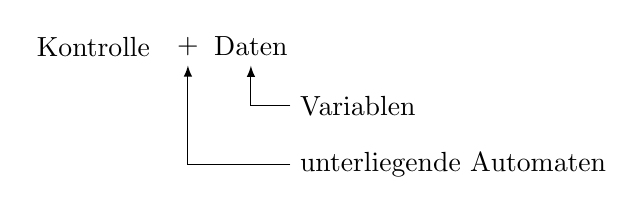
\begin{tikzpicture}
	\node[](kont) at (0,0) {Kontrolle};
	\node[](kont) at (1.2,0) {+};
	\node[](daten) at (2,0) {Daten};
	
	\node[anchor = west](daten_hint) at (2.5,-0.75) {Variablen};
	\node[anchor = west](kont_hint) at (2.5, -1.5) {unterliegende Automaten};
	
	\draw[-latex] (kont_hint.west) -| (kont.south);
	\draw[-latex] (daten_hint.west) -| (daten.south);
	\end{tikzpicture}
\end{center}

Wir betrachten Variablen mit \underline{endlichen Wertebereichen} und die Interaktion des Automaten mit Variablen:
\begin{itemize}
	\item Assignments (Wertezuweisungen) \hspace{5mm} $x := e$
	\item Guards (Bedingungen)
	\item[] Transitionen können von Bedingungen an den Wert der Variablen abhängen
	\item Initialisierungen
	\item[] Startwert der Variablen kann festgelegt werden
\end{itemize}

\begin{bsp}[Digi-Code mit höchstens drei Fehlversuchen]
	\mbox{}
	\begin{center}
		\begin{tikzpicture}
		\node[initial, state](1) at (0,0) {$1$};
		\node[state, label = below:{\small \itshape SeenA}](2) at (2,0) {$2$};
		\node[state, label = below:{\small \itshape SeenAB}](3) at (4,0) {$3$};
		\node[state, label = below:{\small \itshape Open}](4) at (6,0) {$4$};
		
		\node[state](error) at (3,-3) {err};
					
		\path[->] 	
		(1) edge [bend left] node [align=center,fill=white] 
		{$A$} (2)
		(2) edge [bend left] node [align=center,fill=white] 
		{$B$} (3)
		(3) edge [bend left] node [align=center,fill=white] 
		{$A$} (4)
		(2) edge [bend left = 25] node [align=center,fill=white] 
		{$C$} (1)
		(3) edge [bend right = 75] node [align=center,fill=white] 
		{$B,C$} (1)
		(1) edge [loop above] node [align=center] 
		{$B,C$} (1)
		(2) edge [loop above] node [align=center] 
		{$A$} (2);
		\end{tikzpicture}
	\end{center}
	\todo{Übergänge ergänzen}
	Die Variable $ctr: \{0,1,2,3\}$ zählt die Anzahl der Fehlversuche; $1,2,3,4$ sind die Kontrollzustände.
\end{bsp}

Ein Automat mit Variablen kann in ein KTS auseinandergefaltet werden.

\begin{bsp}[Digicode mit höchstens drei Fehlversuchen]
	\mbox{}
	\begin{center}
		\begin{tikzpicture}
			\node[state, initial, text width = 1.1cm, align = center](10) at (0,0) {$1$ \\ $ctr=0$};
			\node[state, text width = 1.1cm, align = center](20) at (4,0) {$2$ \\ $ctr=0$};
			\node[state, text width = 1.1cm, align = center](30) at (8,0) {$3$ \\ $ctr=0$};
			\node[state, text width = 1.1cm, align = center](40) at (12,0) {$4$ \\ $ctr=0$};
			
			\node[state, text width = 1.1cm, align = center](11) at (0,-4) {$1$ \\ $ctr=1$};
			\node[state, text width = 1.1cm, align = center](21) at (4,-4) {$2$ \\ $ctr=1$};
			\node[state, text width = 1.1cm, align = center](31) at (8,-4) {$3$ \\ $ctr=1$};
			\node[state, text width = 1.1cm, align = center](41) at (12,-4) {$4$ \\ $ctr=1$};
			
			\node[state, text width = 1.1cm, align = center](12) at (0,-8) {$1$ \\ $ctr=2$};
			\node[state, text width = 1.1cm, align = center](22) at (4,-8) {$2$ \\ $ctr=2$};
			\node[state, text width = 1.1cm, align = center](32) at (8,-8) {$3$ \\ $ctr=2$};
			\node[state, text width = 1.1cm, align = center](42) at (12,-8) {$4$ \\ $ctr=2$};
			
			\node[state, text width = 1.1cm, align = center](13) at (0,-12) {$1$ \\ $ctr=3$};
			\node[state, text width = 1.1cm, align = center](23) at (4,-12) {$2$ \\ $ctr=3$};
			\node[state, text width = 1.1cm, align = center](33) at (8,-12) {$3$ \\ $ctr=3$};
			\node[state, text width = 1.1cm, align = center](43) at (12,-12) {$4$ \\ $ctr=3$};
			
			\node[state, text width = 1.1cm, align = center](err3) at (0,-16) {$err$ \\ $ctr=3$};
			\node[state, text width = 1.1cm, align = center](err0) at (4,-16) {$err$ \\ $ctr=0$};
			\node[state, text width = 1.1cm, align = center](err1) at (8,-16) {$err$ \\ $ctr=1$};
			\node[state, text width = 1.1cm, align = center](err2) at (12,-16) {$err$ \\ $ctr=2$};
			
			\path[->]
			(10) edge [] node [align=center,fill=white] {$A$} (20)
			(20) edge [] node [align=center,fill=white] {$B$} (30)
			(30) edge [] node [align=center,fill=white] {$A$} (40)
			
			(11) edge [] node [align=center,fill=white] {$A$} (21)
			(21) edge [] node [align=center,fill=white] {$B$} (31)
			(31) edge [] node [align=center,fill=white] {$A$} (41)
			
			(12) edge [] node [align=center,fill=white] {$A$} (22)
			(22) edge [] node [align=center,fill=white] {$B$} (32)
			(32) edge [] node [align=center,fill=white] {$A$} (42)
			
			(13) edge [] node [align=center,fill=white] {$A$} (23)
			(23) edge [] node [align=center,fill=white] {$B$} (33)
			(33) edge [] node [align=center,fill=white] {$A$} (43)
			
			(10) edge [] node [align=center,fill=white] {$B,C$} (11)
			(11) edge [] node [align=center,fill=white] {$B,C$} (12)
			(12) edge [] node [align=center,fill=white] {$B,C$} (13)
			(13) edge [] node [align=center,fill=white] {$B,C$} (err3)
			
			(20) edge [] node [align=center,fill=white] {$A$} (11)
			(21) edge [] node [align=center,fill=white] {$A$} (12)
			(22) edge [] node [align=center,fill=white] {$A$} (13)
			(23) edge [] node 
				   [align=center,fill=white] {$A$} (err3)
			
			(30) edge [] node 
			       [align=center,fill=white] {$B,C$} (11) 			
			(31) edge [] node 
			       [align=center,fill=white] {$B,C$} (12)
			(32) edge [] node 
			       [align=center,fill=white] {$B,C$} (13)
			(33) edge [] node 
			       [align=center,fill=white] {$B,C$} (err3);
			
		\end{tikzpicture}
	\end{center}
\end{bsp}

\subsubsection*{Allgemeines Vorgehen bei Auseinanderfaltung eines KTS mit Variablen}
Zustände: 
\begin{center}
	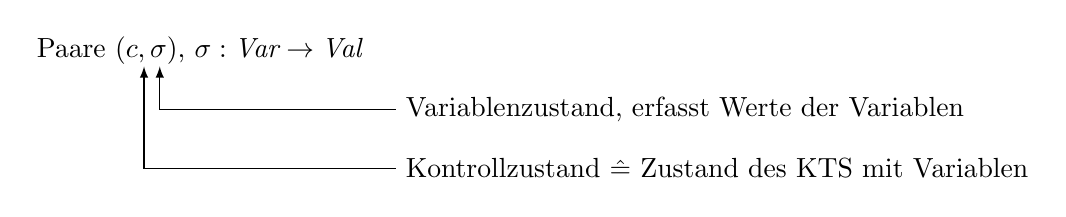
\begin{tikzpicture}
	\node[](zstde) at (0,0) {Paare ($c, \sigma)$, $\sigma: \textit{Var} \rightarrow \textit{Val}$};
	
	\node[anchor = west](var_hint) at (2.5,-0.75) {Variablenzustand, erfasst Werte der Variablen};
	\node[anchor = west](kont_hint) at (2.5, -1.5) {Kontrollzustand \^{=} Zustand des KTS mit Variablen};
	
	\draw[-latex] (kont_hint.west) -| (-0.7,-0.2);
	\draw[-latex] (var_hint.west) -| (-0.5,-0.2);
	\end{tikzpicture}
\end{center}

Transitionen werden nur mit Aktionen benannt. Guards und Assignments werden Start und Zielzustand berücksichtigt. Das auseinandergefaltete KTS enthält Transitionen $((c, \sigma), a, (c', \sigma')$ gdw.

es gibt im ursprünglichen KTS eine mit Aktion $a$, einen Guard $g$ und Assignments $S$ benannte Transition, sodass gilt:
\begin{itemize}
	\item $g$ gilt in $\sigma$
	\item $\sigma'$ ergibt sich durch Anwendung der Effekte der Assignments in $S$ an $\sigma$. ($\sigma' = [[S]](\sigma)$)
\end{itemize}


\begin{bem}[zur Auseinanderfaltung]

	\begin{itemize}
		\item Reduktion des Model-Checking-Problems für Automaten/KTS mit Variablen auf das Problem für reine KTS
		\item Beachte: Auseinanderfaltung hat 
		\[\left(|\textit{Kontrollzustände}| \cdot \prod_{x \text{Variable im \\ gegebenen Automaten/KTC}}\text{Wertebereich von x}\right) \in \Omega\left(2^{\text{Anzahl der Variablen}}\right)\] 
		 viele Zustände. Dies bedeutet regelrecht eine Zustandsexplosion. Mögliche Lösungsansätze sind
		 \begin{itemize}
		 	\item On-the-fly-Model-Checking: Zustandsraum wird inkrementell erzeugt
		 	\item Symbolisches Model-Checking: Mengen von Zuständen mit geeigneten Datenstrukturen kompakt repräsentieren
		 	\item Abstraktion
		 \end{itemize}
	\end{itemize}

	Durch Auseinanderfaltung lassen sich imperative Programme 
	\begin{itemize}
		\item ohne Rekursion (aber mit Schleifen!)
		\item über Variablen mit endlichen Wertebereichen
	\end{itemize}
	im Prinzip behandeln (while-Programme mit endlich-wertigen Variablen). Sie kann in Automaten mit Variablen übersetzt werden.
	\todo{Bild einfügen}
	
	Bei Variablen mit unendlichen Wertebereichen kann eine Abstraktion auf ein Programm mit Variablen über einen endlichen Wertebereich verwendet werden.
\end{bem}

\subsection{Trace- und Bisimulationsäquivalenz von Kripke-Transitionssystemen}
Sei $AP$ eine (endl.) Menge atomarer Präpositionen.

\begin{defn}[Läufe]
	Sei $\mathcal{K} = (S, S_0, \textit{Act}, R, L)$ ein KTS.
	\begin{enumerate}[a)]
		\item Ein endlicher \emph{Lauf} von $\mathcal{K}$ ist eine endliche alternierende Folge $s_0 a_1 s_1 a_2 \dots a_n s_n$ aus Zuständen $s_i \in S$ und Aktionen $a_i \in \textit{Act}$ mit $(s_i,a_{i+1}, s_{i+1}) \in R$ für $i=1 \dots n-1$ und $s_0 \in S_0$.
		
		\item Einun endlicher Lauf von $\mathcal{K}$ ist eine unendliche alternierende Folge $s_0 a_1 s_1 a_2 \dots$ aus Zuständen $s_i \in S$ und Aktionen $a_i \in \textit{Act}$ mit $(s_i,a_{i+1}, s_{i+1}) \in R$ für $i \in \mathbb{N}_0$ und $s_0 \in S_0$.
		
		\item Ein Lauf heißt \emph{maximal}, wenn er nicht verlängerbar ist, d.h. ein unendlicher Lauf ist immer maximal und ein endlicher Lauf $s_0 a_1 s_1 a_2 \dots a_n s_n$ ist maximal, wenn es kein $a \in \textit{Act}$ und $s \in S$ mit $(s_n, a, s) \in R$ gibt.
	\end{enumerate}
\end{defn}

\begin{bsp}
	\label{bsp:kts-aeq}
	Betrachte
	
	\begin{center}
		\begin{tikzpicture}
			\node[]() at (-2.5, 0.5) {$\mathcal{K}_1$};
			\node[state, initial, label = {[align=left, right, xshift=3mm]B}](0) at (0,0) {0};
			\node[state, label = {[align=left, right, xshift=3mm]A}](1) at (0,-2){1};
			\node[state, label = {[align=left, xshift=-2mm,left]R,W}](2) at (-2,-4){2};
			\node[state, label = {[align=left, xshift=2mm, right]R,W}](3) at (2,-4){3};
			
			\path[->]
				(0) edge [] node [align=center,fill=white] {$M$} (1) 		
				(1) edge [] node [align=center,fill=white] {$K$} (2) 		
				(1) edge [] node [align=center,fill=white] {$T$} (3) 		
				(2) edge [bend left=20] node [align=center,fill=white] {$\tau$} (0) 		
				(3) edge [bend right=20] node [align=center,fill=white] {$\tau$} (0);		
				
			\node[text width = 3cm]() at (5,-2) {$M \hat{=}$ Münze\\$K \hat{=}$ Kaffee\\$T \hat{=}$ Tee\\$\tau \hat{=}$ interner Schritt};
			\node[text width = 3cm]() at (9,-2) {$B \hat{=}$ Bereit\\$A \hat{=}$ Auswahl\\$R \hat{=}$ Reinigen\\$W \hat{=}$ Warten};
		\end{tikzpicture}
	\end{center}
	
	$\pi_1 = 0, M, 1, K, 2, \tau, 0, M, 1$ ist ein endlicher Lauf in $\mathcal{K}_1$.
	
	$\pi_2 = 0, M, 1, T, 3, \tau, 0, M, 1, T, 3, \tau, 0, \dots$ ist ein unendlicher Lauf und maximal.
	
	$\mathcal{K}_1$ hat keine maximalen endlichen Läufe.
	
	\todo{K2 und K3 als Bilder einfügen}
	
	$\pi_3 = 0, M, 1, K, 3, \tau, 0, M, 1$ ist ein endlicher Lauf von $\mathcal{K}_2$, nicht maximal.
	
	$\pi_4 = 0, M, 2, T, 4, \tau, 0, M, 2, T, 4, \tau, 0, \dots$ ist ein unendlicher maximal Lauf von $\mathcal{K}_2$.
	
	$\mathcal{K}_2$ hat keine maximalen endlichen Läufe.
\end{bsp}

\begin{defn}[Traces]
	Sei $\mathcal{K} = (S, S_0, \textit{Act}, R, L)$ ein KTS über $AP$.
	
	\begin{enumerate}[a)]
		\item Ein endlicher (bzw. unendlicher) \emph{Trace} ist eine endliche (bzw. unendliche) alternierende Folge $t=X_0 a_1 X_1 \dots a_k X_k$ (bzw. $t=X_0 a_1 X_1 a_2 \dots$) mit $X_i \subseteq \textit{AP}$ und $a_i \in \textit{Act}$.
		
		\item Sei  $\pi = s_0 a_1 s_1 a_2 \dots a_n s_n$ (bzw. $\pi = s_0 a_1 s_1 a_2 \dots $) eine endliche (bzw. unendliche) alternierende Folge von Zuständen $s_i \in S$ und Aktionen $a_i \in \textit{Act}$. Dann heißt $Tr(\pi) = L(s_0) a_1 L(s_1) \dots a_k L(s_k)$ bzw. $Tr(\pi) = L(s_0) a_1 L(s_1) a_2 L(s_2) \dots$ Trace zu $\pi$.
		
		\item Ein Trace $t$ heißt (maximaler) Trace von $\mathcal{K}$, wenn es einen (maximalen) Lauf $\pi$ von $\mathcal{K}$ mit $t=Tr(\pi)$ gibt.
		
		\item[] Es sei $Tr(\mathcal{K})$ die Menge der maximalen Traces von $\mathcal{K}$, d.h. $Tr(\mathcal{K}) = \{Tr(\pi) \mid \pi \text{ ist maximaler Lauf von } \mathcal{K}\}$
		
		\item Zwei Kripke-Transitionssystem $\mathcal{K}, \mathcal{K}'$ über $AP$ mit gleicher Atkionsmenge heißen \emph{trace-äquivalent} (in Zeichen $\mathcal{K} \equiv_{tr} \mathcal{K}'$) gdw. $Tr(\mathcal{K}) = Tr(\mathcal{K'})$.
	\end{enumerate}
\end{defn}

\begin{lemma}
	Die Relation $\equiv_{Tr}$ ist eine Äquivalenzrelation.
\end{lemma}

\begin{beweis}
	Reflexivität, Symmetrie und Transitivität folgen aus den entsprechenden Eigenschaften von \enquote{$=$}:
	
	\begin{description}
		\item[Reflexivität] $Tr(\mathcal{K}) = Tr(\mathcal{K}) \Rightarrow \mathcal{K} \equiv_{Tr} \mathcal{K}$
		\item[Symmetrie] $\mathcal{K} \equiv_{Tr} \mathcal{K'} \Leftrightarrow^{def} Tr(\mathcal{K}) = Tr(\mathcal{K'}) \Leftrightarrow^{def} Tr(\mathcal{K'}) = Tr(\mathcal{K}) \Leftrightarrow^{def} \mathcal{K'} \equiv_{Tr} \mathcal{K}$
		\item[Transitivität] $\mathcal{K} \equiv_{Tr} \mathcal{K'} \equiv_{Tr} \mathcal{K''} \implies Tr(\mathcal{K}) = Tr(\mathcal{K'}) = Tr(\mathcal{K''}) \implies \mathcal{K} \equiv_{Tr} \mathcal{K''}$
	\end{description}
\end{beweis}

\begin{bsp}
	$\mathcal{K}_1$ und $\mathcal{K}_2$ aus Beispiel \ref{bsp:kts-aeq} sind traceäquivalent: $\mathcal{K}_1 \equiv_{Tr} \mathcal{K}_2$.
\end{bsp}

\begin{defn}[Bisimulation, bisimilar]
	\label{def:bisimulation}
	Seien $\mathcal{K} = (S, S_0, Act, R, L)$ und $\mathcal{K'} = (S', S_0', Act, R', L')$ zwei KTSe über $AP$ mit gleicher Aktionsmenge.
	\begin{enumerate}
		\item Eine Relation $B \subseteq S \times S'$ heißt \emph{Bisimulation} falls $\forall (s, s') \in B$ gilt:
		\begin{enumerate}[a)]
			\item $L(s)=L(s')$
			\item $\forall t \in S, a \in Act:$
			
			$(s,a,t) \in R \Rightarrow \exists t' \in S': (s', a, t') \in R' \wedge (t, t') \in B$
			
			\item $\forall t' \in S', a \in Act:$
			
			$(s',a,t') \in R' \Rightarrow \exists t \in S: (s, a, t) \in R \wedge (t, t') \in B$
		\end{enumerate}
	
	\item Zwei Zustände $s \in S, s' \in S'$ heißen \emph{bisimilar} gdw. es eine Bisimulation $B$ mit $(s, s') \in B$ gibt. Wir schreiben dann $s \sim s'$.
	
	\item $\mathcal{K}$ und $\mathcal{K'}$ heißen bisimilar, in Zeichen $\mathcal{K} \sim \mathcal{K'}$ gdw.
	\begin{itemize}
		\item $\forall s \in S_0 \exists s' \in S_0' : s ~ s'$
		\item $\forall s' \in S_0' \exists s \in S_0 : s ~ s'$
	\end{itemize}
	\end{enumerate}
\end{defn}

\begin{bsp}
	\todo{Grafiken malen (4 Kaffeeautomaten)}
	\begin{itemize}
		\item $\mathcal{K}_1$ und $\mathcal{K}_2$ sind bisimilar
		
		$B= \{(0,0), (1,1), (0,2), (1,3)\}$ ist eine Bisimulation
		
		\item $\mathcal{K}_1$ und $\mathcal{K}_3$ sind bisimilar
		
		$B= \{(0,0), (1,1), (1,2)\}$ ist eine Bisimulation
		
		\item $\mathcal{K}_1$ und $\mathcal{K}_4$ sind nicht bisimilar
		
		Annahme: $\exists$ Bisimulation $B$. Dann muss $(0,0) \in B$ und der Schritt $(0, M, 1) \in R_1$ in $\mathcal{K}_1$ durch $(0, M, 1) \in R_2$ oder $(0, M, 2) \in R_2$ in $\mathcal{K}$ gematcht werden. Von $1$ in $\mathcal{K}_4$ kann aber der Schritt $(1,T,0)$ in $\mathcal{K}_1$ nicht gematcht werden und von $2$ in $\mathcal{K}_4$ kann der Schritt $(1, K, 0)$ nicht gematcht werden.
	\end{itemize}
\end{bsp}

\begin{lemma}
	Die in 2) von Definition \ref{def:bisimulation} eingeführte Relation $\sim \subseteq S \times S'$ ist selbst eine Bisimulation, nämlich die größte Bisimulation (d.h. es gilt $B \subseteq \sim \forall$ Bisimulationen). Es gilt $\sim \bigcup \{B \subseteq S \times S' \mid B \textit{ ist Bisimulation}\}$
\end{lemma}

\begin{beweis}
	\mbox{}
	\begin{itemize}
		\item $\sim \bigcup \{B \subseteq S \times S' \mid B \textit{ ist Bisimulation}\}$ ist eine Umformulierung der Definition.
		\begin{align*}
			&\ s \sim s'\\
			&\iff \exists \textit{ Bisimulation } B \subseteq S \times S' \textit{ mit } (s, s') \in B \\
			&\iff (s, s') \in \bigcup \{B \subseteq S \times S' \mid B \textit{ ist Bisimulation}\}
		\end{align*}
		
		\item $\sim$ ist selbst Bisimulation:
		
		Wir überprüfen die Def. Sei $s \sim s'$. Dann existiert eine Bisimulation $B \subseteq S \times S'$ mit $(s, s') \in B$. Dann folgt
		\begin{enumerate}[a)]
			\item $L(S) = L(S')$ (weil $B$ Bisimulation ist)
			\item Sei $t \in S, a \in Act$ mit $(s, a, t) \in R$. Wegen $(s, s') \in B$ und $B$ Bisimulation ist, existiert $t' \in S'$ mit $(s', a, t') \in R'$ und $(t, t') \in B$. Nach Definition von $\sim$ gilt auch $t \sim t'$.
			\item analog.
		\end{enumerate}
	
	\item Wegen $\sim = bigcup \{B \subseteq S \times S' \mid B \textit{ ist Bisimulation}\}$ gilt $B \subseteq \sim \forall \textit{ Bisimulationen } B$, d.h. $\sim$ ist die größte Bisimulation.
	\end{itemize}
\end{beweis}

\begin{lemma}
	$\sim$ (als Relation auf KTS) ist eine Äquivalenzrelation.
\end{lemma}

\begin{beweis}
	\mbox{}
	\begin{description}
		\item[Reflexivität] Auf gegebenem KTS $\mathcal{K} = (S, S_0, Act, R, L)$ ist $id_s = \{(s,s) \mid s \in S\}$ eine Bisimulation wie man leicht überprüft. Folglich gilt $s \sim s \forall s \in S$. Zu jedem $s \in S_0$ können wir ale $s$ selber wählen mit $s \sim s$. Es folgt $\mathcal{K} \sim \mathcal{K}$.
		
		\item[Symmetrie] Man sieht leicht: Ist $B$ eine Bisimulation zwischen $\mathcal{K}$ und $\mathcal{K'}$, so ist $B^{-1} = \{(s,s')\in S' \times S \mid (s, s') \in B \}$ eine Bisimulation zwischen $\mathcal{K}$ und $\mathcal{K'}$. Man kann sich überlegen, dass dies $\mathcal{K'} \sim \mathcal{K}$ impliziert, falls $\mathcal{K'} \sim \mathcal{K'}$ gilt.
		
		\item[Transitivität] Der Schlüssel zum Beweis ist die Beobachtung: Ist $B$ eine Bisimulation zwischen $\mathcal{K}$ und $\mathcal{K'}$ und $B'$ eine Bisimulation zwischen $\mathcal{K'}$ und $\mathcal{K''}$, so ist $B;B' = \{(s, s'') \in S \times S'' \mid \exists s': (s, s') \in B \wedge (s', s'') \in B'\}$ eine Bisimulation zwischen $K\mathcal{K}$ und $\mathcal{K''}$.
	\end{description}
\end{beweis}
\cleardoubleoddemptypage